\subsection{Benchmark overview}

Across four corpora (MIMIC-III, 4CE, CORAL--Breast, CORAL--Pancreas) and four extraction tasks (entity, assertion status, value+unit as a single field, and date processing with start--end joint correctness), CLINES is benchmarked against rule/lexicon pipelines, transformer encoders, and single-prompt LLMs (Figure~\ref{fig:clines-performance}A--D). CLINES (o3-mini) ranks first on every available task--dataset combination. Relative to the strongest single-prompt LLM baseline in the original benchmark cohort (GPT-4o single-prompt), absolute F1 gains are $+0.21$--$0.33$ for entity extraction, $+0.21$--$0.28$ for assertion status, $+0.27$--$0.38$ for value+unit, and $+0.26$--$0.33$ for date processing. Versus transformer encoders (entity only), CLINES improves F1 by $+0.28$--$0.68$ across datasets. Non-LLM baselines trail on entities and do not produce value+unit or date outputs; among them, only cTAKES yields assertion labels.

\new{All primary F1 comparisons additionally carry 95\% percentile bootstrap confidence intervals ($B=2000$ document-level resamples) and paired-bootstrap, FDR-corrected pairwise tests; the per-field point estimates, full bootstrap CIs, and pairwise test results are tabulated in the Supplementary Materials, where Code-field gains and most assertion/value cells are significant at $p_{\mathrm{FDR}}<0.05$ and date-column differences are not reliably resolvable at the available sample sizes.}

\begin{figure}[H]
  \centering
  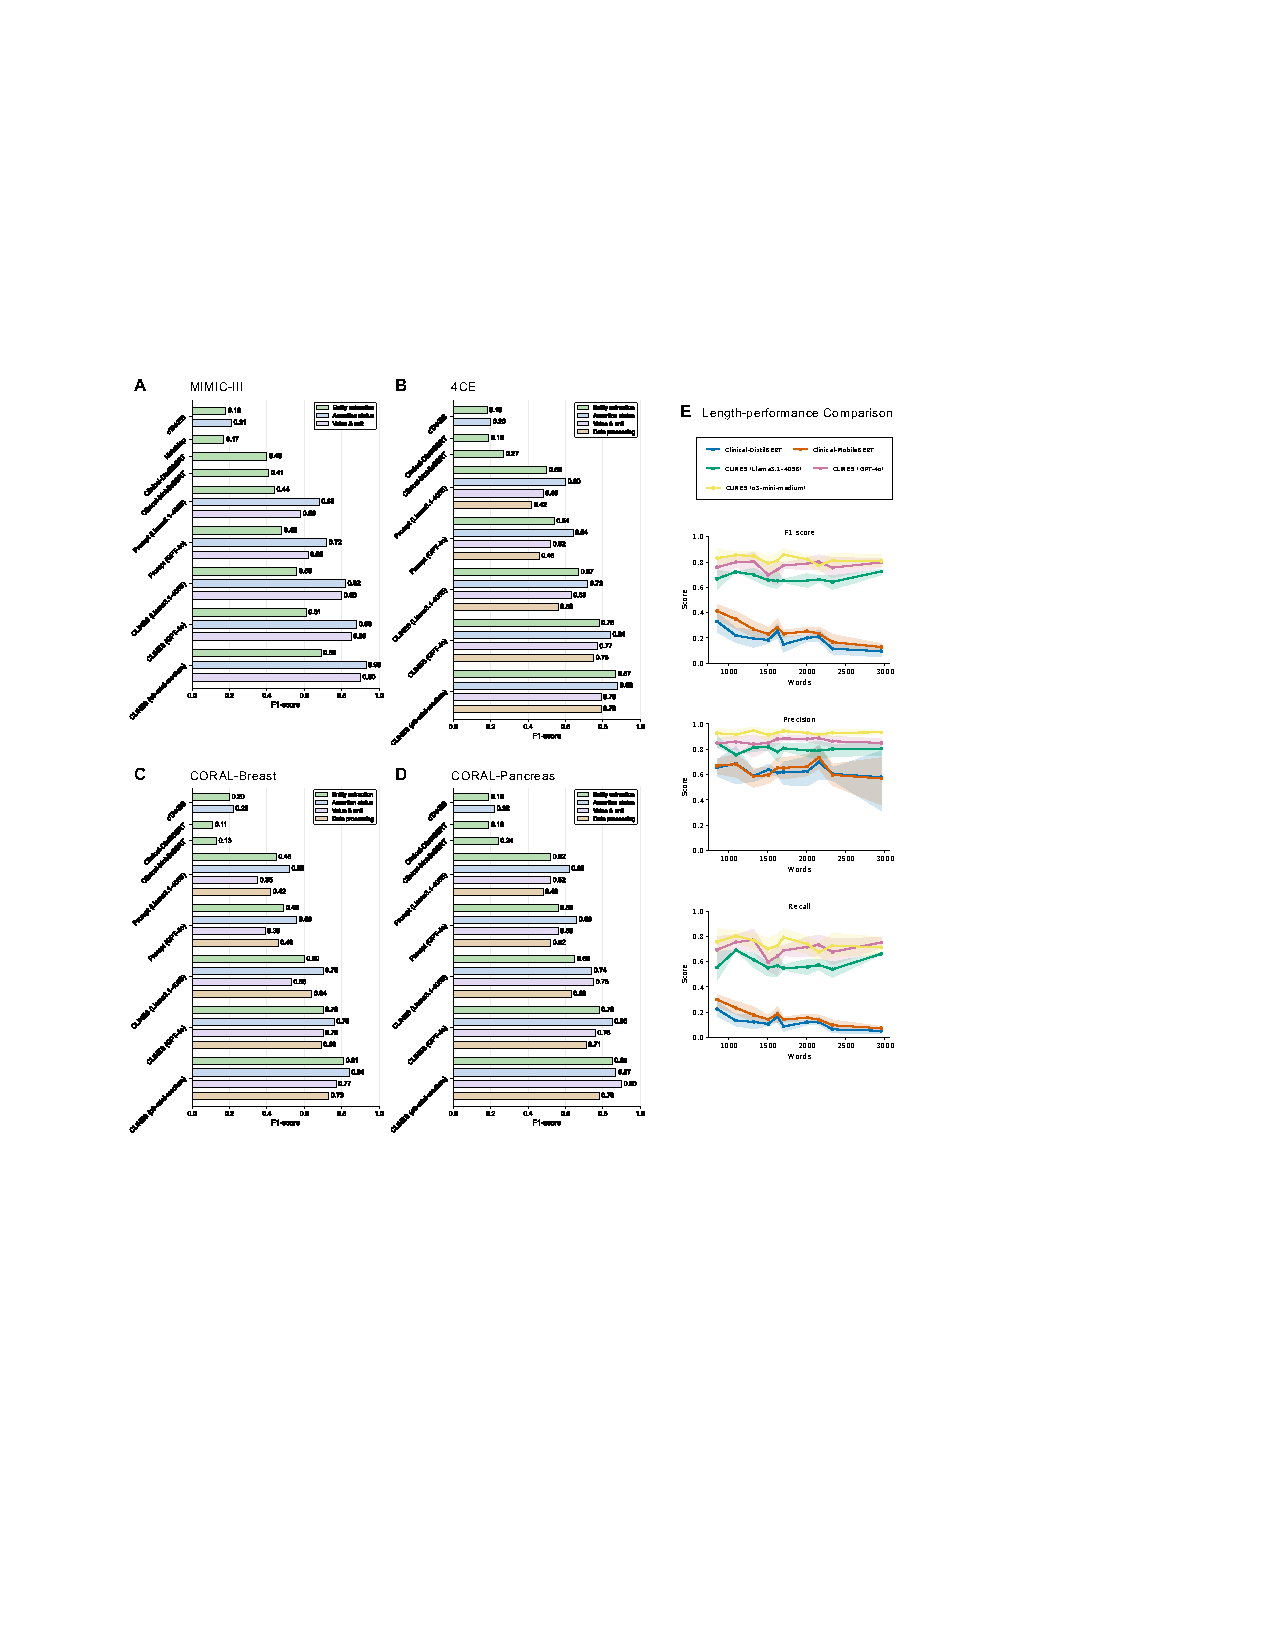
\includegraphics[width=\linewidth]{figures/figure3.pdf}
  \caption{\textbf{Performance of CLINES across datasets and tasks.} (A--D) Results on MIMIC-III, 4CE, and CORAL---Breast/Pancreas comparing CLINES with traditional rule-based NLP, lightweight transformer-based baselines, and LLMs with single-step prompt engineering across six extraction tasks (treating value+unit as a single field and evaluating start+end date as joint correctness). The metric is F1 score. (E) CLINES versus transformer-based baselines as note length/complexity increases, reported as F1, precision, and recall. Notes are grouped into quantile-based length bins; markers indicate the bin-median word count; lines show bin-mean scores; shaded ribbons denote 95\% bootstrap confidence intervals.}
  \label{fig:clines-performance}
\end{figure}


\subsection{Across corpora and variants}

The three CLINES variants maintain a consistent ordering---o3-mini $>$ GPT-4o $>$ Llama-3.1-405B---for entities, assertions, and value+unit, with all three delivering date extraction on 4CE and CORAL. Single-prompt LLMs outperform rule/lexicon and encoder baselines yet remain below CLINES on every task. \new{Quantitatively, hosted GPT-4o trails o3-mini-medium by approximately 10 pp code F1 and the open-weight Llama-3.1-405B trails by approximately 20 pp (Figure~\ref{fig:robustness-cost}A).}

\subsection{Note-length analysis}

Across quantile-based length bins ($\sim$1--3k words), all CLINES variants show stable F1, precision, and recall (Figure~\ref{fig:clines-performance}E). Transformer-encoder baselines decrease with note length and complexity, driven primarily by falling recall, which remains substantially lower than CLINES across bins.

\subsection{\new{Expanded baselines, cost, and ablation}}

\new{Throughout the analyses below we adopt CLINES (o3-mini-medium) as the reference configuration and report the per-field detail on the three consensus-annotated corpora (4CE, CORAL--Breast, CORAL--Pancreas); MIMIC-III is discussed separately because of its single-annotator-per-paragraph protocol. On a cross-annotated subset (three notes per dataset; 2{,}675 candidate-mention rows), pooled mention F1 was 0.82 and assertion Cohen's $\kappa$ was 0.85; a post-stratified analysis of false-positive predictions estimated that 54.3\% were annotation gaps rather than true model errors, with no individual true-hallucination category exceeding 17\% --- full inter-annotator-agreement and hallucination-taxonomy detail are in Supplementary Materials.}

\new{(i) Per-note cost (Figure~\ref{fig:robustness-cost}B): \$0.21 (o3-mini-medium hosted) versus \$0.97 (o3-mini single-prompt) versus $\approx 0.4$ GPU-hours (Llama-3.1-405B FP8, $8\times$H100). (ii) Component ablation (Figure~\ref{fig:robustness-cost}C): SapBERT-based UMLS normalization was load-bearing ($\approx 0.43$ code-F1 loss when removed); cross-chunk reconciliation, semantic chunking, and the date module contributed smaller gains. (iii) Architecture comparison against alternative prompting strategies and off-the-shelf clinical encoders (Figure~\ref{fig:robustness-cost}D): the architecture-attributable gain over o3-mini single-prompt and GPT-4o chain-of-thought was $+0.37$ to $+0.54$ code F1; full-size clinical encoders (BERT-base 110M; GatorTron-base 345M) matched mention detection (F1 0.84--0.89) but emit no normalized codes, assertion, value+unit, or dates.}

\begin{figure}[H]
  \centering
  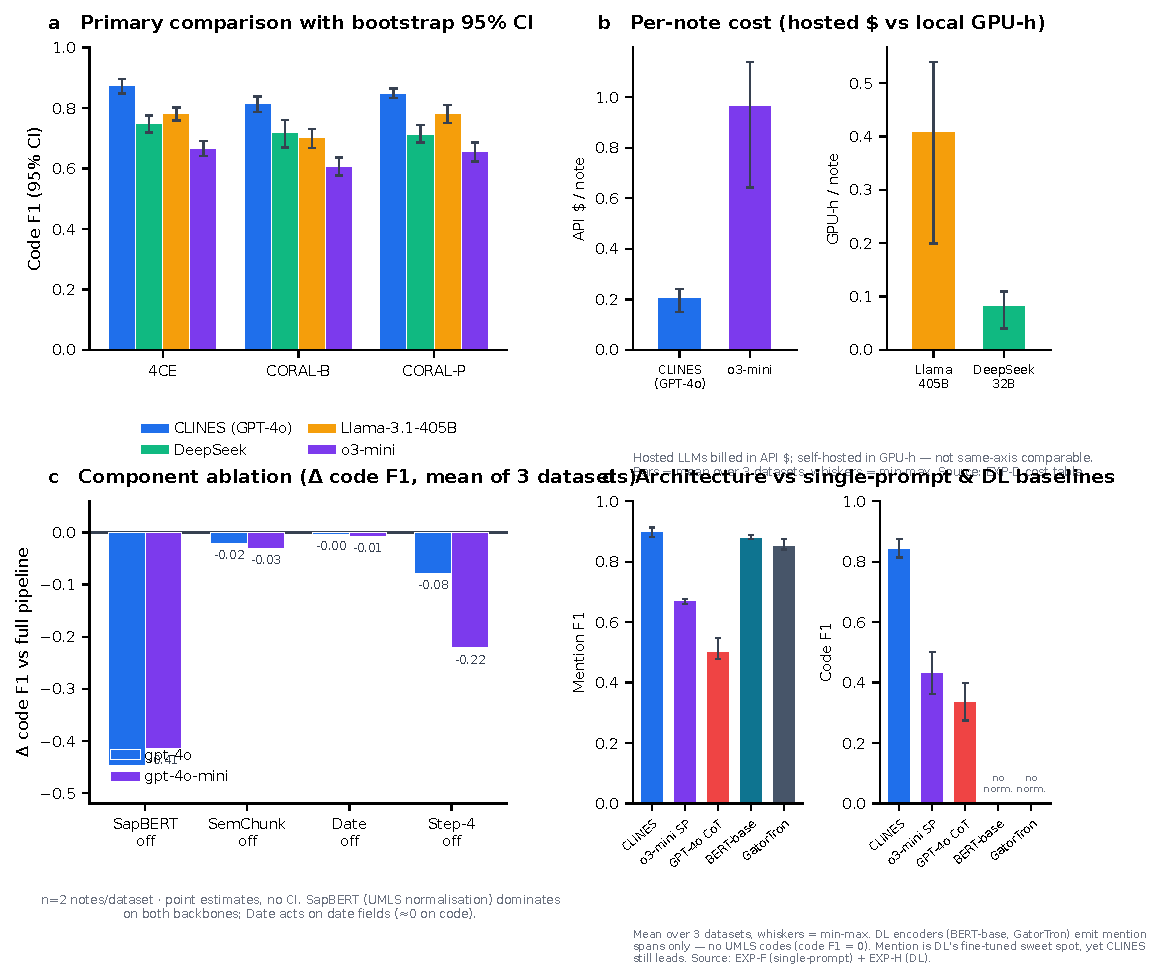
\includegraphics[width=\linewidth]{figures/figure5.pdf}
  \caption{\new{\textbf{Robustness, cost, and component contributions.} (a)~Primary CLINES (GPT-4o) code-F1 comparison against backbone alternatives with 95\% percentile bootstrap confidence intervals. (b)~Per-note cost: hosted-API dollars per note (CLINES (GPT-4o) versus o3-mini) and local GPU-hours per note (Llama-3.1-405B FP8 on 8$\times$H100); the dollar and GPU-hour axes are not directly comparable. (c)~Component ablation (change in code F1 relative to the full pipeline, mean of three datasets) for two backbones (GPT-4o and GPT-4o-mini); removing SapBERT-based UMLS normalization dominates on both backbones. (d)~CLINES versus single-prompt LLM baselines (o3-mini single-prompt, GPT-4o chain-of-thought) and full-size clinical deep-learning encoders (BERT-base clinical NER, GatorTron-base); the encoders emit entity spans only and produce no UMLS codes, so their code F1 is undefined.}}
  \label{fig:robustness-cost}
\end{figure}

